% Originally: content/week-08.tex, \section{Multivariate integration} (Corsin Week 8)

% Source: Corsin Nick/Class Notes/Week 8.pdf, p. 7
\section{Multivariate integration}
\label{sec:multivariate_integration}

% Supplement: Sascha Brack/Class Notes/Week_08_Notes_Monday.pdf, pp. 5--7
\subsection{Jordan measure and the Riemann integral}
The rigorous definition of the multidimensional integral relies on the \newterm{Jordan measure} (\germanterm{Jordan-Maß}). The intuition, as presented in Sascha Brack's notes, involves \qt{dyadic cubes} (pixels) that approximate a region from the inside and outside.

\begin{center}
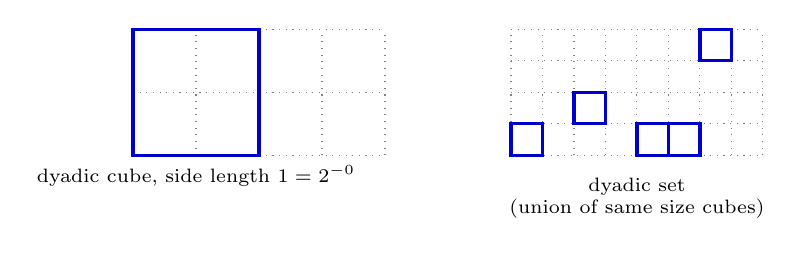
\begin{tikzpicture}[scale=0.8]
  % first grid
  \draw[gray, dotted] (0,0) grid (4,2);
  \draw[very thick, blue!80!black] (0,0) rectangle (2,2);
  \node[below, font=\scriptsize] at (1,0) {dyadic cube, side length $1=2^{-0}$};
  
  \begin{scope}[shift={(6,0)}]
    \draw[gray, dotted, step=0.5] (0,0) grid (4,2);
    \draw[very thick, blue!80!black] (0,0) rectangle (0.5,0.5);
    \draw[very thick, blue!80!black] (1,0.5) rectangle (1.5,1.0);
    \draw[very thick, blue!80!black] (2,0) rectangle (2.5,0.5);
    \draw[very thick, blue!80!black] (2.5,0) rectangle (3.0,0.5);
    \draw[very thick, blue!80!black] (3,1.5) rectangle (3.5,2.0);
    \node[below, font=\scriptsize, align=center] at (2,-0.2) {dyadic set\\(union of same size cubes)};
  \end{scope}
\end{tikzpicture}
\end{center}

Similar to the 1D Riemann integral, we approximate the volume of a set $E \subseteq \mathbb{R}^n$ using an outer sequence of dyadic sets $G_i \supseteq E$ and an inner sequence $F_i \subseteq E$. If the limits of their volumes coincide as the pixel size $2^{-p} \to 0$, $E$ is \newterm{Jordan measurable}.

Furthermore, the multidimensional integral of a non-negative function $f : A \to \mathbb{R}$ is exactly the $(n+1)$-dimensional Jordan measure (volume) of its hypograph $\Gamma_A(f)$:

\begin{center}
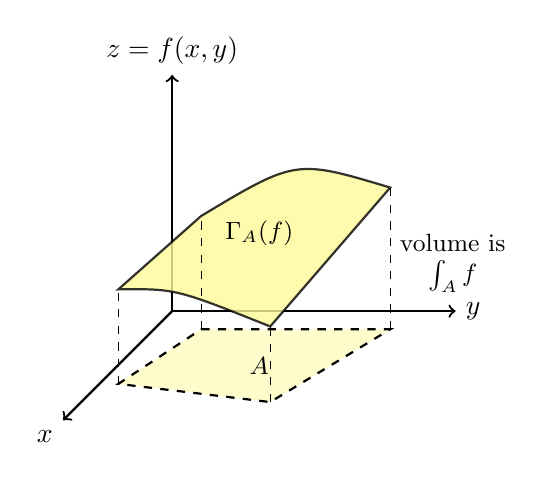
\begin{tikzpicture}[scale=1.2]
  % axes
  \draw[->, thick] (0,0,0) -- (3,0,0) node[right] {$y$};
  \draw[->, thick] (0,0,0) -- (0,2.5,0) node[above] {$z = f(x,y)$};
  \draw[->, thick] (0,0,0) -- (0,0,3) node[below left] {$x$};
  
  % base domain A
  \draw[thick, dashed, fill=yellow!20] (0.5,0,0.5) -- (2.5,0,0.5) -- (2.0,0,2.5) -- (0.2,0,2.0) -- cycle;
  \node[font=\small] at (1.5, 0, 1.5) {$A$};
  
  % top surface graph(f)
  \draw[thick, fill=yellow!40, opacity=0.8] (0.5,1.2,0.5) .. controls (1.5,1.8,0.5) .. (2.5,1.5,0.5)
    -- (2.0,0.8,2.5) .. controls (1.0,1.2,2.5) .. (0.2,1.0,2.0) -- cycle;
  \node[font=\small] at (1.5, 1.4, 1.5) {$\Gamma_A(f)$};
  
  % vertical lines
  \draw[dashed] (0.5,0,0.5) -- (0.5,1.2,0.5);
  \draw[dashed] (2.5,0,0.5) -- (2.5,1.5,0.5);
  \draw[dashed] (2.0,0,2.5) -- (2.0,0.8,2.5);
  \draw[dashed] (0.2,0,2.0) -- (0.2,1.0,2.0);
  
  \node[right, font=\small, align=center] at (2.5, 0.7, 0.5) {volume is\\$\int_A f$};
\end{tikzpicture}
\end{center}


% --- exercises relocated here from the dissolved sheet 8 ---

% Originally: content/week-08.tex, \exercisesheet{8}, problem 8.2
% Source: exercises/Ex8_Analysis2_eng.pdf

% Source: exercises/Ex8_Analysis2_eng.pdf, p. 1
\begin{exercise}[8.2 --- True or False \textnormal{(important)}]
\label{ex:8.2}
\begin{enumerate}[label=\textbf{\arabic*.}]
  \item A bounded countable set is always Jordan-null.
  \item A countable set is always Lebesgue-null.
  \item Let $D \subset [0,1]$ be a dense set (i.e.\ $\overline D = [0,1]$). Then
    $\mu_{out}(D) = 1$. ($\mu_{out}$ was defined in Definition 13.10.)
  \item Let $X, Y \subset [0,1]$ Jordan measurable sets such that $\mu(X) > 1/2$ and
    $\mu(Y) > 1/2$. Then $X \cap Y \neq \emptyset$.
  \item Let $X, Y \subset [0,1]$ such that $\mu_{out}(X) > 1/2$ and $\mu_{out}(Y) > 1/2$. Then
    $X \cap Y \neq \emptyset$.
\end{enumerate}
\textit{Official hint:} \textbf{8.2.5} --- $\mu_{out}$ can be positive and large on very sparse
sets\dots

% Supplement: Sascha Brack/Ex Sheet Hints/Ex8_Analysis2_hints.pdf, p. 1
\textit{Sascha Brack's hints:} a toolkit of sets worth testing every part against ---
$\mathbb{Q}$, the irrationals $\mathbb{R}\setminus\mathbb{Q}$, $\mathbb{Q}\cap[0,1]$, and
$(\mathbb{R}\setminus\mathbb{Q})\cap[0,1]$. For \textbf{8.2.3} specifically: monotonicity already
gives $\mu_{out}(D) \leq \mu_{out}([0,1]) = 1$, so the work is showing
$\mu_{out}(D) \geq 1$ --- essentially, that the \qt{smallest} dyadic set containing $D$ also
contains $[0,1]$.
\end{exercise}

% Originally: content/week-08.tex, \exercisesheet{8}, problem 8.4
% Source: exercises/Ex8_Analysis2_eng.pdf

% Source: exercises/Ex8_Analysis2_eng.pdf, p. 1
\begin{exercise}[8.4 --- Multiple Choice \textnormal{(important)}]
\label{ex:8.4}
Let $U \subset \mathbb{R}^n$ be a nonempty, open subset, $f : U \to \mathbb{R}^m$ a function,
and $N \subset U$ a Jordan null set. In which of the following cases is the image
$f(N) \subset \mathbb{R}^m$ necessarily a null set? \textit{Attention: Only one answer is
correct!}
\begin{enumerate}[label=\textbf{\arabic*.}]
  \item If $f$ is uniformly continuous.
  \item If $f$ is uniformly continuous and $m \geq n$.
  \item If $f$ is locally Lipschitz continuous.
  \item If $f$ is locally Lipschitz continuous and $m \geq n$.
\end{enumerate}
\end{exercise}
